
%* FULL PAPER EXAMPLE FOR CODAWORK'17 *********
\documentclass [10pt]{article}

%* some useful packages *********
\usepackage{amsfonts,amssymb,amsmath}
\usepackage{epsfig,chicago,float}
\usepackage[ansinew]{inputenc}
\usepackage[]{graphicx}

\bibliographystyle{chicago}
%****************************************************************
\setlength{\oddsidemargin}{+4.6mm}
%
\setlength{\textwidth}{15cm}
%
\setlength{\textheight}{23cm}
%
\setlength{\topmargin}{-1.25cm} \setlength{\baselineskip}{1mm}
%
\setlength{\parindent}{0pt}
%
\setlength{\parskip}{0.25cm}
%
\pagestyle{empty}
%
\renewcommand{\refname}{\centerline{REFERENCES}}
%
%*for Spanish*************************************************
\newcommand{\enye}{\~n}
%**************************************************************


%*for captions*******************************************
\renewcommand{\figurename}{\footnotesize{\bf Figure}}
\renewcommand{\tablename}{\footnotesize{\bf Table}}
%*****************************************************


%****************the document **************************

\begin{document}
\begin{center}
\textbf{\large Instructions for authors - CoDaWork 2017}

\vskip 0.25cm

\textbf{Jia R. Wu}$^{1}$\textbf{, Jean M. Macklaim}$^{1}$\textbf{, and
Gregory B. Gloor}$^{1,2}$ \\
{\small $^{1}$Dep't of Biochemistry, U. Western Ontario, London, Canada, N6A 5C1\\
$^{2}$Dep't of Applied Mathematics, U. Western Ontario, London, Canada, N6A 5C1 \\
\textit{gbgloor@gmail.com} \\
}
\end{center}

\vskip 0.5cm {\centerline{\bf Abstract}}

High throughput sequencing is a technology that allows for the generation of millions of reads of genomic data regarding a study of interest, and data from high throughput sequencing platforms are usually count compositions. Subsequent analysis of this data can yield information on transcription profiles, microbial diversity, or even cellular abundance in culture. These data have many pathologies: because of the high cost of acquisition the data are usually sparse, and often contain far fewer observations than variables. However, an under-appreciated pathology of these data are their often unbalanced nature: i.e, there is often be systematic variation between groups simply due to presence or absence of features, and this variation is important to the biological interpretation of the data. A simple example would be comparing transcriptomes of yeast cells with and without a gene knockout. This causes samples in the comparison groups to exhibit widely varying centres. Despite the compositional nature of sequencing data, the majority tools inappropriately model the the underlying features in sequencing data as linearly independent counts. This work extends a previously described log-ratio transformation method that allows for variable comparisons between samples in a compositional context. We demonstrate the pathology in several modelled and real unbalanced experimental designs that have a unidirectional direction of change to show how this dramatically causes both false negative and false positive inference in both traditional and compositional approaches. We then introduce several measures drawn from the RNA-seq and robust CoDa analysis fields to demonstrate how the pathologies can be addressed. An extreme example is presented where only the use of a predefined basis is appropriate. The transformations are implemented as an extension to a general compositional data analysis tool known as ALDEx2 or ANOVA Like Differential Expression. 

{\bf Key words: } ALDEx2, Bayesian estimation, sparse data, high throughput sequencing, robust estimation, qPCR

\vskip 1cm

\newpage

\section{Introduction}
\vskip-0.25cm High throughput sequencing (HTS) technology is used to generate information regarding the relative abundance of features.  In these designs, DNA or RNA is isolated, a library is made from a  sample of the nucleic acid, and a random sample of the library is sequenced on an instrument. The output is a set of short sequence tags, called reads, which are mapped to example sequences for each feature to generate a table of read counts per feature for every sample. Traditionally, samples comprise a set of features whose identity depends on the experimental design. For example, features are genes in the case of RNA-seq or  metagenomic sequencing, or are operational taxonomic units (OTUs) when the objective is identifying microbial diversity. 

These data are often analyzed by count based methods, such as negative binomial or zero-inflated Gaussian models, that assume the features are independent and identically distributed for statistical tests \shortcite{Auer:2010aa,Anders:2013aa}. However,  the capacity of the instrument used for HTS imposes an arbitrary upper limit on the total number of reads observed. Thus, data collected from high throughput sequencing are compositions, and so counts per feature are not independent when collected in this way. Traditional tools do not address the compositional nature of HTS data \shortcite{fernandes:2014,gloorAJS:2016} and assume that the features are sufficiently independent when there are enough of them, or when they fulfill certain statistical properties \shortcite{Weiss:2016aa}, although much effort is placed on `normalizing' the data to have a consistent read depth \shortcite{Sun:2013aa,McMurdie:2014a}.

Formally, \shortciteN{Aitchison:1986} defined a composition as a vector \textit{\textbf{x}}  of positive values \textit{x1}\ldots\textit{xD} whose components  sum to an arbitrary constrained constant \textit{c}. The constant sum is usually set to 1, leading to these vectors being of unit length. Absolute values of components in a composition are uninformative, and the only information provided in compositional data are the relative magnitudes of the ratios between the pairs of components, and Aitchison demonstrated that compositional data  can be efficiently analyzed by log-ratios between the parts, since these data carry only relative information between components \shortcite{Aitchison:1986}.

One way of satisfying the need to examine the ratios between parts is to use the centered-log-ratio (CLR) transformation proposed by Aitchison, defined as: 

\begin{equation}
\begin{split}
clr_x &= log  \big( \frac{x_i}{g(x)}   \big)_{i=1,\dots,D} \\
\text{where}~
	clr_x &= \text{A composition transformed by CLR} \\
	x_i &= \text{A feature of the non-transformed composition (x)} \\
	D &= \text{The number of features of x} \\ 
	g(x) &= \text{Geometric mean of D features of x}
\end{split}
\label{eq:CLR}
\end{equation}

Since all arbitrary sums are the same this led to the concept of a composition as an equivalence class where composition \textit{\bf{x}} can be scaled into an identical composition \textit{\textbf{y}} by multiplication of a constant $\alpha$ \shortcite{barcelo:2001}. Thus, we can discuss any composition as being a proportion scaled by $\alpha$ without loss of precision. The CLR, and indeed any ratio-based method is scale-invariant because if the parts of \textit{\textbf{x}} are counts with $\alpha=$\textit{N} reads, then: 
\begin{equation}
	clr_x= log\big( \frac{Nx_i}{g(Nx)}   \big) =  log\big( \frac{x_i}{g(x)}  \big).
\label{eq:equip}
\end{equation}

For convenience, the analyses and discussion here are drawn from RNA-seq, or transcriptome, experiments where the data are exploring the relative abundance of gene species that are found in cells in an environment. However, the results and conclusions apply without restriction to metagenomic sequencing, microbial diversity sampling (by 16S rRNA gene sequencing) or to in-vitro selection experiments \shortcite{fernandes:2014}. 

\subsubsection{Sparsity and asymmetry in HTS data}
\vskip-0.25cm
It is common for HTS data to be sparse, that is, for a given sample to contain features with one or more counts of 0. Furthermore, the sparsity of the samples is affected by the total number of reads obtained for each sample. It is common for samples in a transcriptome to contain thousands of features each of which may have a dynamic range of over 4 logs. In many cases a transcriptome dataset will be composed of several groups, where the expression of a gene (feature) is so low that it is below the detection limit in one group, and very high in another group. The expression of genes in biological systems is linked, and some genes control the expression of other genes, either by increasing or decreasing their relative abundance. Furthermore, the cell has a built-in control system whereby gene expression itself appears to be a composition, that is, the expression levels of all genes in a cell are constrained by an absolute upper bound  \shortcite{Scott:2010}. Note however, that this does not mean that a population of cells will have total gene expression with an upper bound, since the cells themselves can change in both absolute and relative abundance in a mixture. 

The potential for a change in cell number and the potential for expression linkage of genes in biological systems, coupled with the inability to collect a large enough number of sequence reads, can lead to experiments with an apparent or a real asymmetry in relative abundance of many genes or features. Such an asymmetry will result in a mis-centering of the data when conducting differential abundance analyses, largely, but not exclusively because of the effect on the geometric mean upon which the CLR depends. 

\section{Statement of the Problem}
\vskip-0.25cm

The assumption being made when using the CLR transformation to identify features that vary between groups is that most features are either invariant or varying at random. This assumption is broken if there is any sort of systematic variation between groups. For example, when comparing microbial diversity between sampling sites or conditions, organisms present in one sub-site or condition may be absent from another \cite{Macklaim:2015aa,Hummelen:2010,Gajer:2012}. In the case of multi-organism RNA-seq (meta-rna-sea), organisms that reside in one condition may have a different expression profile and abundance than those that reside in a second condition \cite{macklaim:2013}. In the case of a single-organism RNA-seq, samples from one condition may contain more genes than samples from another condition \cite{Lang:2015aa,Peng:2014aa,Zhao:2013aa}. These differences are represented by either zeroes or low count features that occur in only one group. 

It will be demonstrated that exaggerated differences can be achieved with seemingly little variation within simulated data. Additionally, zeroes are problematic as they cannot be represented in logarithmic space. Therefore, prior to the log ratio transformation, zero count features are discarded if present in exclusive or conditions, or adjusted with an uninformative prior. The goal is to identify a non-deterministic geometric mean that best represents each sample so features can be accurately compared.

\subsection{Simulated Data}
\vskip-0.25cm
RNA-Seq data was simulated for benchmarking purposes. Assemblies from \textit{Saccharomyces cerevisiae} uid 128 and  a complete reference genome of \textit{S. cerevisiae} were drawn from GenBank. The R package \texttt{polyester v1.10.0} was used to simulate an RNA-Seq experiment with 2 groups of 10 replicates with 20x sequencing coverage across the simulation experiment. For the base dataset, forty genes were chosen at random to have 2-5 fold expression difference, and these were apportioned equally between the two groups. These 40 features serve as an internal control of true positives for each dataset as their fold changes are explicit and should always be displayed as differentially expressed. We used bowtie2 to align the simulated reads  to the \textit{S. cerevisiae} reference genome. Labeling each group as A and B is arbitrary and hence samples s\_1, s\_2, ..., s\_10 belong to condition A, and samples s\_11, s\_12, ..., s\_20 belong to condition B. There are a total of 6349 features in these simulated data, and only the first 1000 genes were chosen for the majority of the figures. On average, samples in the unmodified base dataset have a simulated read depth of approximately 870000 reads. 

An additional 98 datasets derived from the base dataset are generated in order to benchmark how well the IQR (robust?) log-ratio transformation supports the assumption that most features are invariant and unchanging. As the original dataset has approximately 6000 nonzero features, 60 features are incrementally removed from the samples of condition A in each simulated dataset for a resultant set of datasets with sparsity ranging from 0\% to 98\% sparse in condition A. 

\subsection{An illustration}
\vskip-0.25cm
In its current implementation, ALDEx2 computes a per-sample geometric mean for the features and declares this as the baseline for feature comparisons. Figure~\ref{Fig:f1a}:symmetric is an effect plot demonstrating that the 40 internal control features are found to be both statistically significant and to have an effect size greater than 1 between the two groups, and the remainder of the features have very small difference, and correspondingly have an effect size much less than 1. The inset histogram shows the distribution of difference values between groups A and B, and it is clear that it is symmetric and has a location of 0. However, the introduction of small amounts of asymmetry strongly affect the results. The asymmetric 2\% dataset is the base dataset modified by setting the count value to 0 for 20 features chosen at random from Group A, and likewise the asymmetric 6\% dataset has 60 features from group A set to 0. It is apparent from the two right panels of Figure ~\ref{Fig:f1b} that this low level of simulated asymmetry breaks the assumption that most features are invariant, and the location of the difference between groups is no longer at the origin. Supplementary Figure 1 shows compositional biplots of the same data, and here it is obvious that the centre of the data is not at the origin. Thus, the small amount of asymmetry is shifting the geometric mean of the data, causing bias. Thus, if there are a large proportion of features in a sample that do not follow the central tendency of the data, the geometric mean can be unreliable as a baseline. It is unlikely that the problem will be as easy to diagnose in real data as in simulated data. 

\begin{figure}[ht]
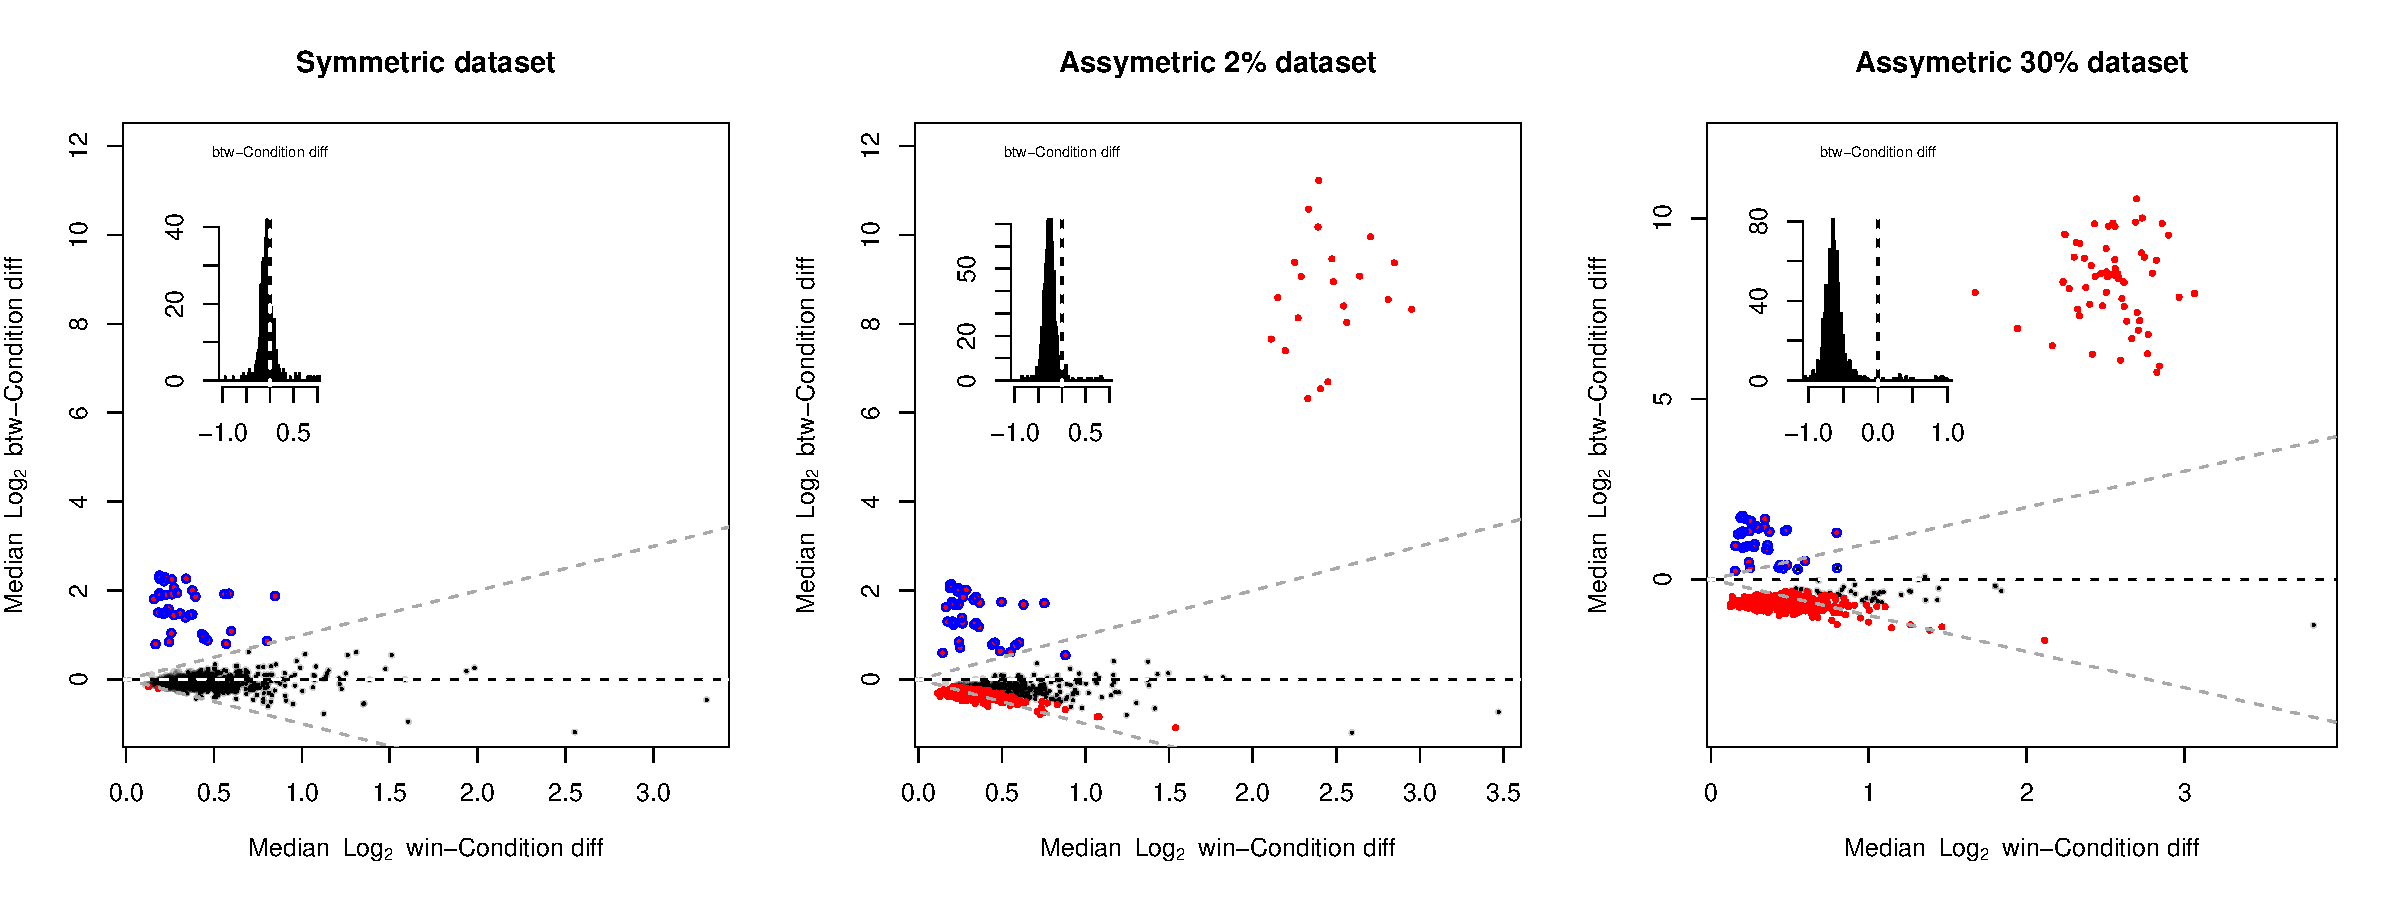
\includegraphics[width=6in]{../figures/Fig_1.pdf}
\vspace{3mm} \caption{Effect plots of simulated asymmetric data that illustrates the problem. The effect plots show the difference between two conditions simulated RNA-seq data with 1000 genes and 40   }
\label{Fig:f1a}
\end{figure}

As can be seen in Equation \ref{eq:CLR}, the major determinant of the centre of a sample is the denominator, or basis, used to compute the CLR. Thus, one obvious approach to solving the problem is to compute the geometric mean of a subset of features that are better representative of the central tendency of the data, and to use this value as the denominator in the equation. We next examined four different approaches to identifying the features to include in the denominator. 

The first approach was to identify those features that have variance that is most typical across all the samples. This was  done by calculating the variance of each feature after CLR transformation of the data, then using those features with a variance between the first and third quartiles of the dataset when calculating the geometric mean of the features. This transformation is termed the CLR\textsubscript{iqlr}, transformation, since the denominator for Equation \ref{eq:CLR} is the features from the inter-quartile range of the variance. The results of this method are shown in Figure \ref{Fig:f2a}:IQLR, for the sake of brevity, only the effect on the Asymmetric 2\% dataset is illustrated, but below, we explore the limitations of this, and other transformations. 

\begin{figure}[ht]
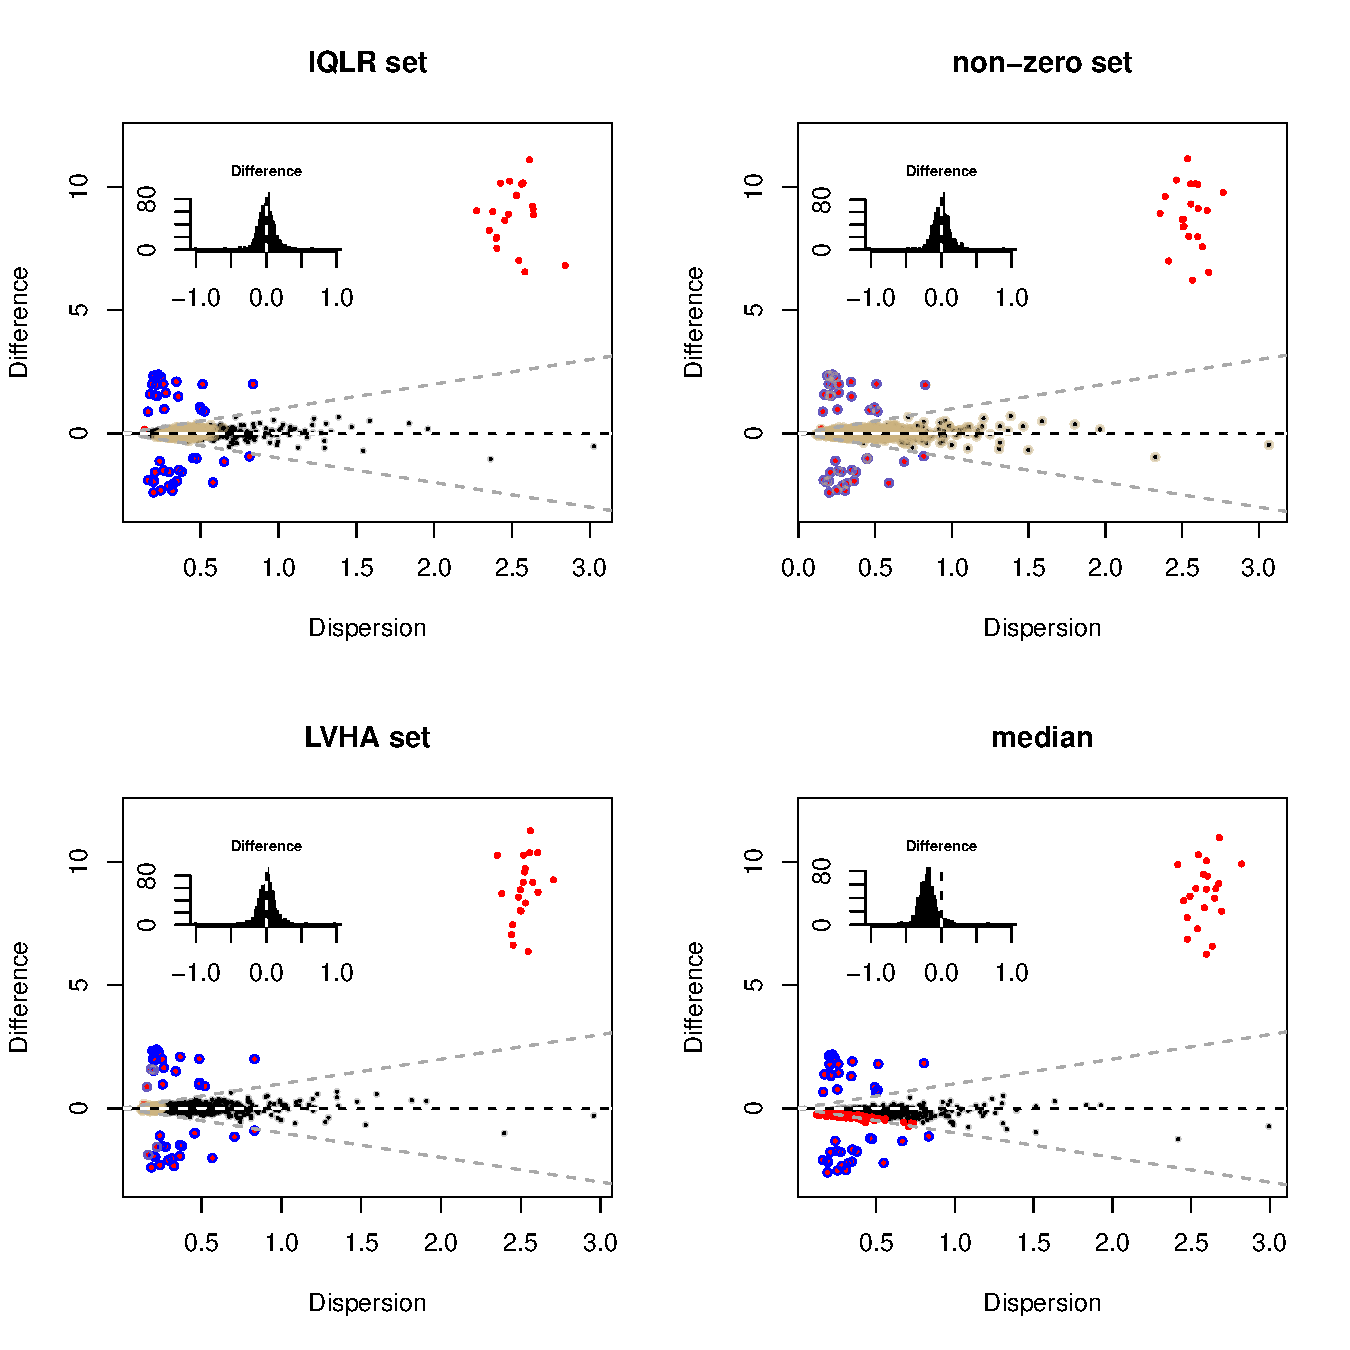
\includegraphics[width=6in]{../figures/Fig_2.pdf}
\vspace{3mm} \caption{Effect plots of simulated asymmetric data with transformations, based on the CLR that can result in a more accurate centring of the data.   }
\label{Fig:f2a}
\end{figure}

Remember that the final electronic paper --without limit in the number of pages-- will be due {\bf before May 4,
2017}. It will be sent in PDF format. It will be published in the CoDaWork'17 CD (with ISBN) and will be available in
the sessions of the workshop. {\bf Only papers of participants registered before May 4, 2017 will be included in the
proceedings CD}.

\section{First level headings}
\vskip-0.25cm The workshop on Compositional Data is intended as a
forum for discussion of important points related to the
statistical treatment and modelling of compositional data, as well
as their applications and interpretation. The goal of such
discussions is to get some insight into the most appealing future
lines of research in the field.

\subsection{Second level headings}
\vskip-0.25cm
In order to meet this general but clear goal, we
intend to bring together a significant number of specialists,
users and interested people to collect critical contributions and
start a stimulating brainstorming.

\subsubsection{Third level headings}
\vskip-0.25cm The Introductory course to statistical analysis of
compositional data will work from a variety of practical
compositonal problems. Different case studies will be presented
and analyzed using CoDaPack, a freeware software based on EXCEL.
This software is oriented to users coming from the applied
sciences. No extensive background in using computer packages is
required.


\section{Citations, figures and references}
\vskip-0.25cm
\subsection{Citations in text}
\vskip-0.25cm
Citations within the text should include the
author's last name and year: ``The air conditioner data (Proschan,
1963) ...", or when the author is used as a noun in the sentence:
``Proschan (1963) presented a data set ...".

In text, captions, and table headings, list all authors if two or
fewer, and just the first author followed by ``and others" for
more. Examples:

\begin{center}
(Jones and Johnson, 1986; Emmanuel and others, 1989)
\end{center}
or
\begin{center}
Emmanuel and others (1989) showed that ..., whereas Jones and
Johnson (1986) found that ...
\end{center}

When giving a quote or referring to a specific fact or formula in
a book or from an article of more than 8 pages, the citation
should include the page number. Examples:

\begin{center}
(Chayes, 1956, p. 55) or (Matheron, 1975, p. 229).
\end{center}

Page numbers should not be given in the text when referring to the
work as a whole. As with figures, you do not need to direct the
reader to ``see" a citation to the literature. Be sure your
references are accurate and formatted correctly.

\subsection{Figures}
\vskip-0.25cm
All figures should be inserted within the text
exactly as they should appear when printed. All figures must be
centered. Figure number and caption always appear below the
figure. Leave 2~line spaces between the figure and the caption.

\begin{figure}[ht]
\vspace{3mm} \caption{This is a figure caption.}
\end{figure}

When you refer to an illustration, capitalize and spell out the
word ``Figure" if not in parenthesis, as in \ \ ``Figure 2 shows
that the distribution of permeability is skewed ..."; or
abbreviate if in parenthesis, as in \ \  ``The distribution of
permeability is skewed (Fig. 2) ...".

If you have multiple parts in a figure, then label them with
capital letters A,B,C, etc. Refer to them in the text as Figure
2A, or (Fig. 2A). In captions, follow this example:


\begin{figure}[ht]
\vspace{3mm} \caption{Density functions: (A) Permeability; (B)
Porosity.}
\end{figure}


\subsection{Tables}
\vskip-0.25cm
All tables must be centered, neat, clean, and
legible. Table number and title always appear above the table (see
the example below). Use one line space before the table title, one
line space after the table title, and one line space after the
table.

\begin{table}[ht]
\caption{This is an example of a table.}
\begin{center}
\begin{tabular}{lr}
Income         &$\$ 42.94$ \\ Expenses       &$\$ 26.12$ \\ \hline
Rest           &$\$ 16.82$ \\ \hline \hline
\end{tabular}
\end{center}
\end{table}

The word ``Table" should be capitalized, and not abbreviated even
in parentheses.

\subsection{Equations}
\vskip-0.25cm
The word ``Equation" should be capitalized and
spelled out in the text, as in ``It follows from Equation (3) that
..." but capitalized and abbreviated in parenthesis, as in ``It
follows [Eq. (3)] that ...". If you use any other word to refer to
an equation, such as ``expression" or ``relationship", do not
capitalize.



\section*{Acknowledgements and appendices}
\vskip-0.25cm
Use non-numbered first level headings for the
acknowledgements. They should follow text, and precede the list of
references. Appendices follow references, and should be headed
``{\bf Appendix} A" etc. if more than one.

\section*{References}

\bibliography{bibdesk_refs}
%
%\vskip-0.25cm References follow the acknowledgements. Use first
%level no-numbered headings. The bibliography should follow the
%{\it Chicago style}. See below for examples.
%
%\vspace{0.5mm}
%\hangindent=0.5cm \hangafter=1 %
%Ghahramani, Z. (1997).
%\newblock Learning dynamic Bayesian networks.
%\newblock In C.~Giles and M.~Gori (Eds.), {\em Adaptive Processing of Sequences
%  and Data Structures}, Lecture Notes in Artificial Intelligence, pp.\
%  168--197. Berlin: Springer Verlag.
%
%\hangindent=0.5cm \hangafter=1 %
%Pearl, J. (1986).
%\newblock Fusion propagation and structuring in belief networks.
%\newblock {\em Artificial Intelligence\/}~{\em 29\/}(3), pp. 241--288.
%
%\hangindent=0.5cm \hangafter=1 %
%Whittaker, J. (1990).
%\newblock {\em Graphical models in applied multivariate statistics}.
%\newblock Chichester: Wiley.

\end{document}
